% !TEX root = ../presentation.tex
% !BIB program = biber
% !TEX program = xelatex


\section{Out-of-distribution detection}
% \subsection{Out-of-distribution detection}

\frame{
    \frametitle{Defining OOD detection}
    \begin{columns}

    \begin{column}{0.5\textwidth}
        
    Out-of-distribution (OOD) detection is about enabling models to distinguish the training data distribution $p(\xb)$ from any other distribution $\tilde{p}(\xb)$.

    \vspace{3mm}

    We are concerned with doing this on a per-observation basis, i.e. answering the question:

    \vspace{3mm}
    
    \begin{center}
        "Was $\xb$ sampled from $p(\xb)$ or not?"
    \end{center}
    
    \vspace{3mm}
    
    % It is related to \textbf{anomaly detection} and \textbf{adversarial example detection}.
    \end{column}
    
    \begin{column}{0.5\textwidth}

    \begin{figure}[\textwidth]
        \centering
        \begin{tikzpicture}
        \begin{axis}[
          domain=0:13,samples=100,
          height=4.5cm, width=8cm,
          xtick=\empty,
          every axis plot/.append style={very thick,smooth}
        ]
        
        \addplot [name path=p1, color=red!50!black] {gauss(5,1)};
        \addplot [name path=p2, color=black] {gauss(8,1)};
        \path[name path=axis] (axis cs:0,0) -- (axis cs:10,0);
        \addlegendentry{$p(\xb)$}
        \addlegendentry{$\tilde{p}(\xb)$}

        \end{axis}
        \end{tikzpicture}
    \end{figure}
    \begin{figure}[\textwidth]
        \centering
        \begin{tikzpicture}
        \begin{axis}[
          domain=0:13,samples=100,
          height=4.5cm, width=8cm,
          every axis plot/.append style={very thick,smooth}
        ]
        
        \addplot [name path=p1, color=red!50!black] {gauss(4,0.5)};
        \addplot [name path=p2, color=black] {gauss(9,0.5)};
        \path[name path=axis] (axis cs:0,0) -- (axis cs:10,0);
        \addlegendentry{$p(\xb)$}
        \addlegendentry{$\tilde{p}(\xb)$}
        
        \end{axis}
        \end{tikzpicture}
    \end{figure}
    \end{column}
    
    \end{columns}
}


\frame{
    \frametitle{Problem and Contributions}
    \begin{itemize}
        \item Deep generative models often fail at OOD detection task when using their likelihood estimate as the score function \cite{nalisnick_deep_2019} by, perhaps surprisingly, assigning \textbf{higher likelihoods} to the OOD data.
        \item Contributions:
        \begin{itemize}
            \item We present a fast and fully unsupervised method for OOD detection competitive with the state-of-the-art
            \item We provide evidence that out-of-distribution detection fails due to learned low-level features that generalize across datasets.
        \end{itemize}  
    \end{itemize}
}


\frame{
    \frametitle{In distribution?}
    \begin{figure}[\textwidth]
        \centering
        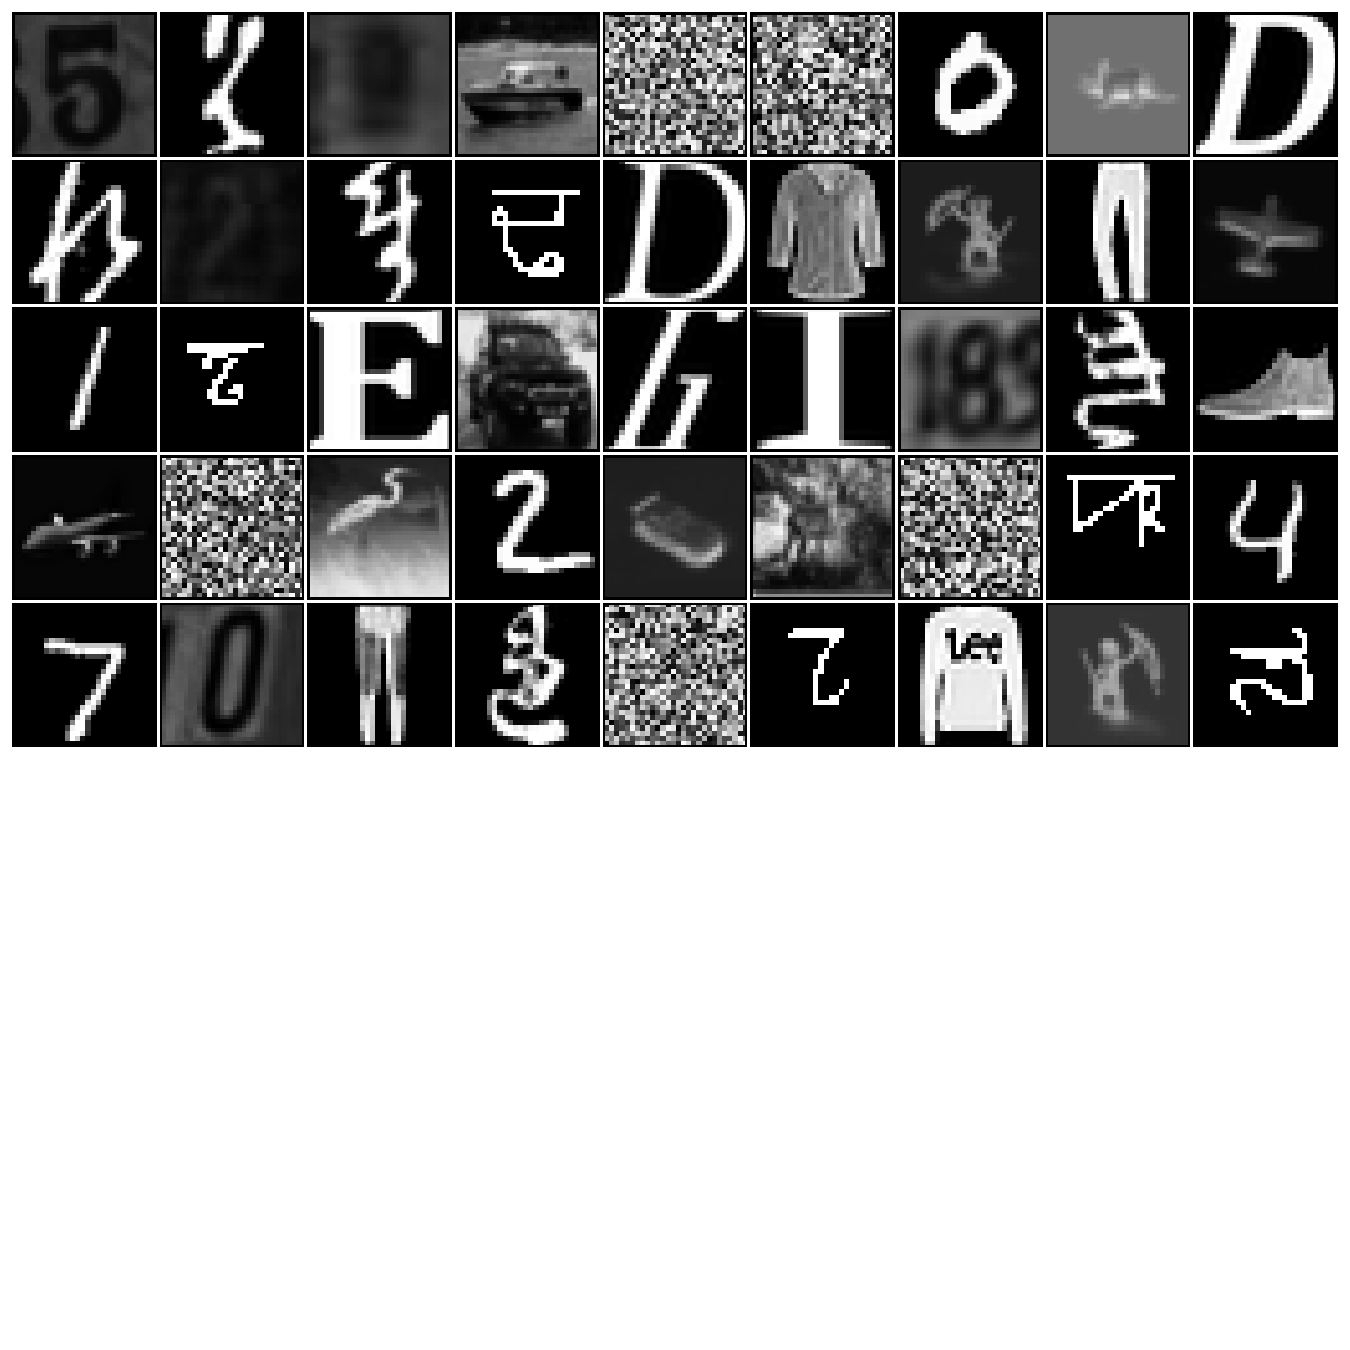
\includegraphics[scale=0.6]{figures/dataexamples_shuffled.pdf}
    \end{figure}
}


\frame{
    \frametitle{Out of distribution?}
    \begin{figure}[\textwidth]
        \centering
        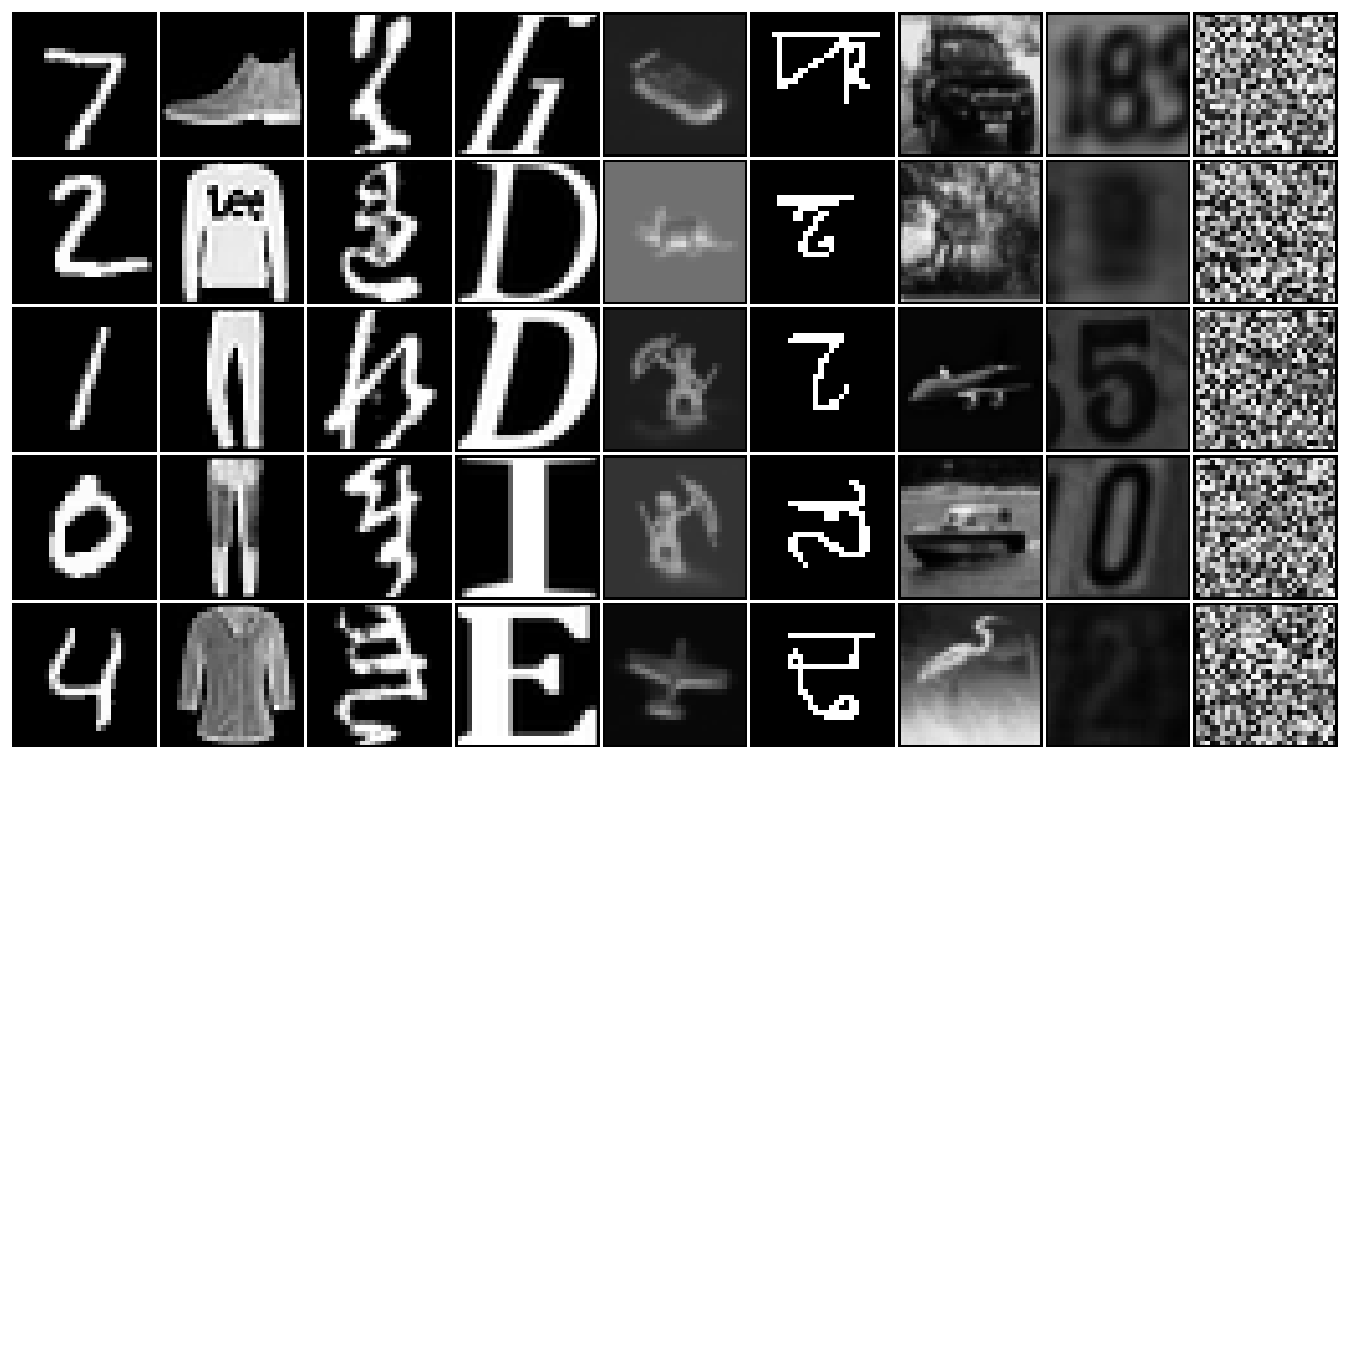
\includegraphics[scale=0.6]{figures/dataexamples.pdf}
    \end{figure}
}



\section{Latent variable models}

\begin{frame}{Hierarchical VAE}
  \begin{columns}
      \begin{column}{0.7\textwidth}
          We choose the hierarchical VAE as our model \cite{kingma_autoencoding_2014, rezende_stochastic_2014}.
          \begin{equation*}
              p_\theta(\xb) = \int p_\theta(\xb,\zb) \text{d}\zb = \int p_\theta(\xb|\zb)p_\theta(\zb) \text{d}\zb
          \end{equation*}
          Specifically we use
          
          \begin{enumerate}
              \item a three-layered hierarchical VAE with bottom-up inference and deterministic skip-connections for both inference and generation.
              \begin{align*}
                  \text{Generative model: }\quad p_\theta(\xb|\zb) &= p_\theta(\xb|\zb_1) p_\theta(\zb_1|\zb_2) p(\zb_3),\\
                  \text{Inference model: }\quad q_\phi(\zb|\xb) &= q_\phi(\zb_1|\xb)q_\phi(\zb_2|\zb_1)q_\phi(\zb_3|\zb_2).
              \end{align*}
              \item a ten-layered layered Bidirectional-Inference Variational Autoencoder (BIVA) \cite{maaloe_biva_2019}.
          \end{enumerate} 
      \end{column}
      \begin{column}{0.3\textwidth}
          \begin{figure}[.5\textwidth]
          \tikz{
          % inference
          % nodes
          \node[obs] (x_inf) {$\xb$};%
          \node[latent,above=.75cm of x_inf](z1_inf){$\zb_1$}; %
          \node[latent,above=.75cm of z1_inf](z2_inf){$\zb_2$}; %
          \node[latent,above=.75cm of z2_inf](z3_inf){$\zb_3$}; %
          \node[above=of z3_inf, yshift=-1.cm] (phi) {$q_\phi(\zb|\xb)$}; 
          
          % edges
          \edge[]{x_inf}{z1_inf};
          \edge[]{z1_inf}{z2_inf};
          \edge[]{z2_inf}{z3_inf};
          \edge[dashed, bend left]{x_inf}{z2_inf};
          \edge[dashed, bend left]{x_inf}{z3_inf};
          
          % generative
          % nodes$
          \node[obs,right=0.75cm of x_inf] (x_gen) {$\xb$};%
          \node[latent,above=.75cm of x_gen](z1_gen){$\zb_1$}; %
          \node[latent,above=.75cm of z1_gen](z2_gen){$\zb_2$}; %
          \node[latent,above=.75cm of z2_gen](z3_gen){$\zb_3$}; %
          \node[above=of z3_gen, yshift=-1.cm] (theta) {$p_\theta(\xb,\zb)$}; 
          
          % edges
          \edge[]{z3_gen}{z2_gen};
          \edge[]{z2_gen}{z1_gen};
          \edge[]{z1_gen}{x_gen};
          \edge[dashed, bend left]{z2_gen}{x_gen};
          \edge[dashed, bend left]{z3_gen}{x_gen};
          }
          \end{figure}
      \end{column}
  \end{columns}
\end{frame}



\section{Identifying the issue}


\frame{
    \frametitle{What is wrong with the ELBO for OOD detection?}
    We can split the ELBO into two terms
    \begin{equation}
        \mathcal{L}(\xb;\theta,\phi) 
        = \mathbb{E}_{q_\phi(\zb|\xb)} \left[ \log \frac{p_\theta(\xb,\zb)}{q_\phi(\zb|\xb)} \right] 
        = \underbrace{\mathbb{E}_{q_\phi(\zb|\xb)}[\log p_\theta(\xb|\zb)]}_{\text{reconstruction likelihood}} - \underbrace{D_{\mathrm{KL}}( q_\phi(\zb|\xb) || p(\zb))}_{\text{regularization penalty}} \ .
    \end{equation}
    The first term is high if the data is well-explained by $\zb$.

    \vspace{3mm}
    The second term we can rewrite as,
    \begin{equation}
        D_{\mathrm{KL}}( q_\phi(\zb|\xb) || p(\zb)) = \mathbb{E}_{q_\phi(\zb|\xb)} \Big[ \textstyle\sum_{i=1}^{L-1} \log \frac{p_\theta(\zb_i|\zb_{i+1})}{q_\phi(\zb_i|\zb_{i-1})} + \log \frac{p_\theta(\zb_L)}{q_\phi(\zb_L|\zb_{L-1})} \Big] \ .
    \end{equation}
    The absolute log-ratios grow with $\mathrm{dim}(\zb_i)$ since the log probability terms are computed by summing over the dimensionality of $\zb_i$.
    
    \vspace{3mm}
}


\frame{
    \frametitle{What do the lowest latent variables code for?}
    
    Absolute Pearson correlations between data representations in all layers of the inference network of a hierarchical VAE trained on FashionMNIST and of another trained on MNIST. 
    \vspace{0.3cm}

    Correlation computed between the representations of the two different models given the same data, FashionMNIST (top) and MNIST (bottom).
    
    \begin{figure}[\textwidth]
        \centering
        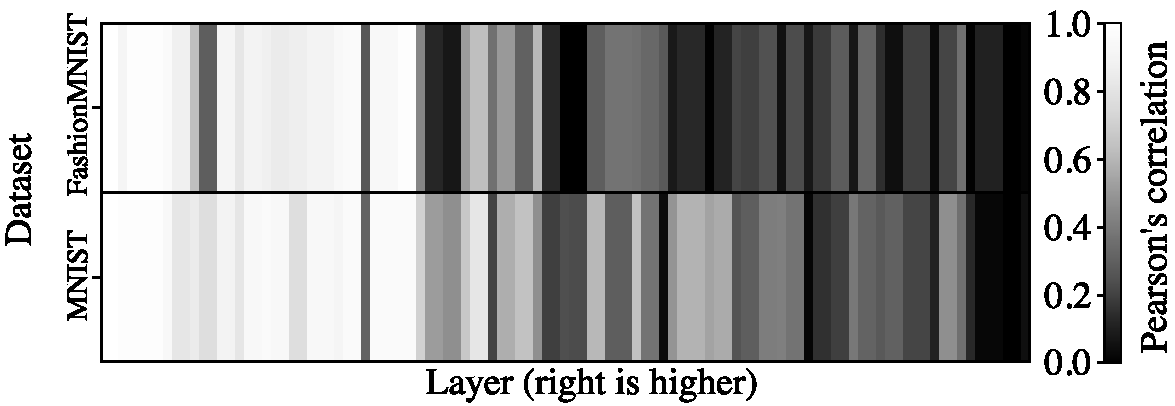
\includegraphics[scale=0.75]{../graphics/paper_hierarchical/feature-correlation-heatmap2.pdf}
        % \caption{Caption}
        % \label{fig:my_label}
    \end{figure}
}


\section{The $\mathcal{L}^{>k}$ likelihood bound}


\frame{
    \frametitle{An alternative likelihood bound, $\mathcal{L}^{>k}$}
    An alternative version of the ELBO that only partially uses the approximate posterior can be written as \cite{maaloe_biva_2019}
    \begin{equation}
        \mathcal{L}^{>k}(\xb; \theta, \phi) = \mathbb{E}_{p_\theta(\zb_{\leq k}|\zb{>k})q_\phi(\zb_{>k}|\xb)} \left[ \log \frac{p_\theta(\xb|\zb)p_\theta(\zb_{>k})}{q_\phi(\zb_{>k}|\xb)} \right]
    \end{equation}
    
    Here, we have replaced the approximate posterior $q_\phi(\zb|\xb)$ with a different proposal distribution that combines part of the approximate posterior with the conditional prior, namely
    
    $$p_\theta(\zb_{\leq k}|\zb_{>k})q_\phi(\zb_{>k}|\xb)$$
    
    This bound uses the conditional prior for the lowest latent variables in the hierarchy.
}


\section{Likelihood ratio}


\frame{
    \frametitle{Likelihood ratios}
    We can use our new bound to compute the score used in a standard likelihood ratio test \cite{buse_likelihood_1982}.
    \begin{equation}\label{eq:llr-as-difference-in-likelihoods}
        LLR^{>k}(\xb) \equiv \mathcal{L}(\xb) - \mathcal{L}^{>k}(\xb) \ .
    \end{equation}
    We can inspect what this likelihood-ratio measures by considering the exact form of our bounds.
    \begin{align}
        \mathcal{L}      &= \log p_\theta(\xb) - D_{\mathrm{KL}}\left( q_\phi(\zb|\xb) || p_\theta(\zb|\xb)\right), \label{eq:likelihoods-as-exact} \\ 
        \mathcal{L}^{>k} &= \log p_\theta(\xb) - D_{\mathrm{KL}}\left( p_\theta(\zb_{\leq }|\zb_{>k}) q_\phi(\zb_{>k}|\xb) || p_\theta(\zb|\xb)\right) \notag \ .
    \end{align}
    In the likelihood ratio the reconstruction terms cancel out and only the KL-divergences from the approximate to the true posterior remain.
    \begin{align}\label{eq:llr-as-kls}
        LLR^{>k}(\xb) &= - D_{\mathrm{KL}}\left( q_\phi(\zb|\xb) || p_\theta(\zb|\xb)\right) \\
                     &\quad + D_{\mathrm{KL}}\left( p_\theta(\zb_{\leq }|\zb_{>k}) q_\phi(\zb_{>k}|\xb) || p_\theta(\zb|\xb)\right) \ . \notag
    \end{align}
}


\frame{
    \frametitle{Importance sampling the ELBO}
    The well-known importance weighted autoencoder (IWAE) bound is tight with the true likelihood in the limit of infinite samples, $S\rightarrow\infty$ \cite{burda_importance_2016},
    \begin{equation}\label{eq:iw-bound}
        \mathcal{L}_{S} = \mathbb{E}_{q(\zb|\xb)}\left[ \log \frac{1}{N} \sum_{s=1}^{S} \frac{p(\xb, \zb^{(s)})}{q(\zb^{(s)}|\xb)} \right] \leq \log p_\theta(\xb) \ ,
    \end{equation}

    \vspace{3mm}

    Consequently, by importance sampling the ELBO, the associated KL-divergence associated vanishes and our likelihood ratio reduces to the KL-divergence associated with $\mathcal{L}^{>k}$.

    \begin{equation}\label{eq:llr-as-kls-iwae-reduced}
        LLR^{>k}_{S}(\xb) \rightarrow D_{\mathrm{KL}}( p(\zb_{\leq }|\zb_{>k}) q(\zb_{>k}|\xb) || p(\zb|\xb)) \ .
    \end{equation}

    We can now see that $LLR^{>k}_{S}(\xb)$ performs OOD detection based on the top-most latent variables.
}


\frame{
    \frametitle{Results with $LLR^{>k}$}
    \begin{figure}[\textwidth]
    \centering
    \begin{subfigure}[c]{0.49\textwidth}
        \centering
        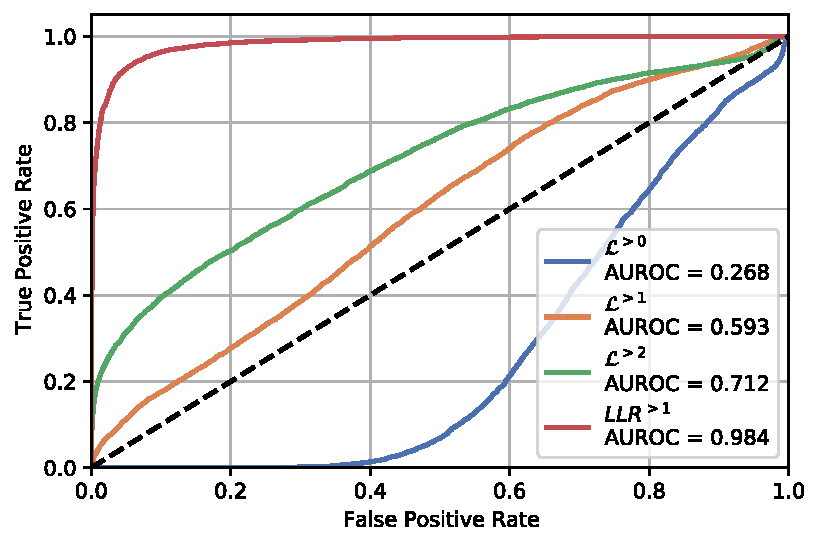
\includegraphics[width=\textwidth]{../graphics/paper_hierarchical/roc-FashionMNIST-test-MNIST-test-ll-and-llr-IW250_sohau.pdf}
        \caption{FashionMNIST HVAE evaluated on MNIST}
    \end{subfigure}
    \hfill
    \begin{subfigure}[c]{0.49\textwidth}
        \centering
        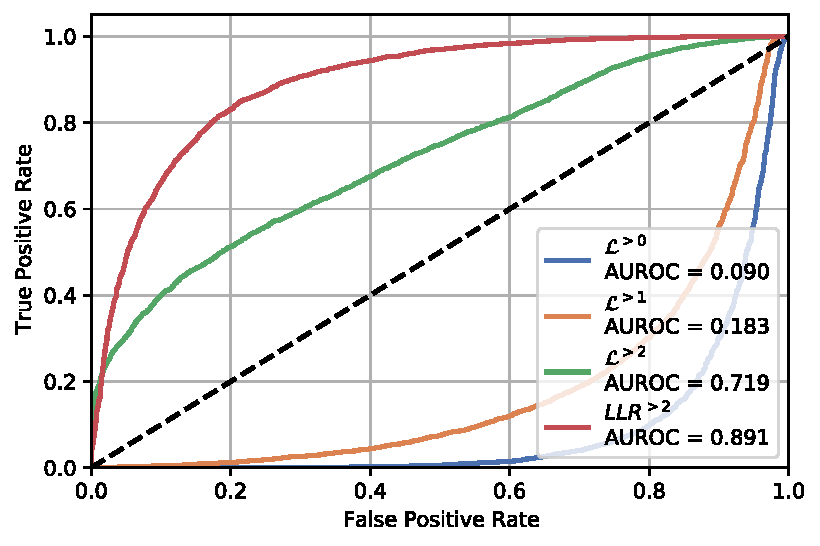
\includegraphics[width=\textwidth]{../graphics/paper_hierarchical/roc-biva-CIFAR10-SVHN-ll-and-llr_sohau.pdf}
        \caption{CIFAR10 BIVA evaluated on SVHN}
    \end{subfigure}
    \end{figure}
}


\frame{
    \frametitle{Results with $LLR^{>k}$}
    The score has good performance across many datasets.

    \begin{columns}

    \begin{column}{0.5\textwidth}

        \begin{table}[t]
            \centering
            \resizebox{0.9\textwidth}{!}{%
            \begin{tabular}{llrrr}
                \toprule
                 OOD dataset & Metric & AUROC$\uparrow$ & AUPRC$\uparrow$ & FPR80$\downarrow$ \\
                 \midrule
                 \multicolumn{5}{c}{\textbf{Trained on CIFAR10}} \\
                 \midrule
        SVHN          &  $LLR^{>2}$  &  0.811  &  0.837  &  0.394  \\
        CIFAR10       &  $LLR^{>1}$  &  0.469  &  0.479  &  0.835  \\
                 \midrule
                 \multicolumn{5}{c}{\textbf{Trained on SVHN}} \\
                 \midrule
        CIFAR10            &  $LLR^{>1}$       &  $0.939$  &  $0.950$  &  $0.052$  \\
        SVHN               &  $LLR^{>1}$       &  $0.489$  &  $0.484$  &  $0.799$  \\
            \bottomrule
            \end{tabular}
            }
        \end{table}
    \end{column}
    
    \begin{column}{0.5\textwidth}
        \begin{table}[t]
            \centering
            \resizebox{0.9\textwidth}{!}{%
            \begin{tabular}{llrrr}
                \toprule
                 OOD dataset & Metric & AUROC$\uparrow$ & AUPRC$\uparrow$ & FPR80$\downarrow$ \\
                 \midrule
                 \multicolumn{5}{c}{\textbf{Trained on FashionMNIST}} \\
                 \midrule
        MNIST                    & $LLR^{>1}$             &  0.986  &  0.987  &  0.011 \\
        notMNIST                 &  $LLR^{>1}$            &  0.998  &  0.998  &  0.000 \\
        KMNIST                   &  $LLR^{>1}$            &  0.974  &  0.977  &  0.017 \\
        Omniglot28x28            &  $LLR^{>2}$            &  1.000  &  1.000  &  0.000 \\
        Omniglot28x28Inverted    &  $LLR^{>1}$            &  0.954  &  0.954  &  0.050 \\
        SmallNORB28x28           &  $LLR^{>2}$            &  0.999  &  0.999  &  0.002 \\
        SmallNORB28x28Inverted   &  $LLR^{>2}$            &  0.941  &  0.946  &  0.069 \\
        FashionMNIST             &  $LLR^{>1}$            &  0.488  &  0.496  &  0.811 \\
                 \midrule
                 \multicolumn{5}{c}{\textbf{Trained on MNIST}} \\
                 \midrule
        FashionMNIST                   &  $LLR^{>1}$  &  $0.999$  &  $0.999$  &  $0.000$ \\
        notMNIST                       &  $LLR^{>1}$  &  $1.000$  &  $0.999$  &  $0.000$ \\
        KMNIST                         &  $LLR^{>1}$  &  $0.999$  &  $0.999$  &  $0.000$ \\
        Omniglot28x28                  &  $LLR^{>1}$  &  $1.000$  &  $1.000$  &  $0.000$ \\
        Omniglot28x28Inverted          &  $LLR^{>1}$  &  $0.944$  &  $0.953$  &  $0.057$ \\
        SmallNORB28x28                 &  $LLR^{>1}$  &  $1.000$  &  $1.000$  &  $0.000$ \\
        SmallNORB28x28Inverted         &  $LLR^{>1}$  &  $0.985$  &  $0.987$  &  $0.000$ \\
        MNIST                          &  $LLR^{>2}$  &  $0.515$  &  $0.507$  &  $0.792$ \\
                 \bottomrule
            \end{tabular}
            }
            % \caption{Additional results for the HVAE model trained on FashionMNIST. All results computed with 1000 importance samples.}
            % \label{tab:additional-results-fashionmnist}
        \end{table}
    \end{column}

    \end{columns}
}


% \frame{
%     \frametitle{Results with $LLR^{>k}$}
%     % The score has good performance across many different datasets.
    
%     \begin{columns}

%     \begin{column}{0.5\textwidth}

%         \begin{table}[t]
%             \centering
%             \resizebox{0.6\textwidth}{!}{%
%             \begin{tabular}{llr}
%                 \toprule
%                  OOD dataset & Metric & AUROC$\uparrow$ \\
%                  \midrule
%                  \multicolumn{3}{c}{\textbf{Trained on CIFAR10}} \\
%                  \midrule
%         SVHN          &  $LLR^{>2}$  &  0.811 \\
%         CIFAR10       &  $LLR^{>1}$  &  0.469 \\
%                  \midrule
%                  \multicolumn{3}{c}{\textbf{Trained on SVHN}} \\
%                  \midrule
%         CIFAR10            &  $LLR^{>1}$       &  0.939 \\
%         SVHN               &  $LLR^{>1}$       &  0.489 \\
%             \bottomrule
%             \end{tabular}
%             }
%         \end{table}
%     \end{column}
    
%     \begin{column}{0.5\textwidth}
%         \begin{table}[t]
%             \centering
%             \resizebox{0.75\textwidth}{!}{%
%             \begin{tabular}{llr}
%                 \toprule
%                  OOD dataset & Metric & AUROC$\uparrow$ \\
%                  \midrule
%                  \multicolumn{3}{c}{\textbf{Trained on FashionMNIST}} \\
%                  \midrule
%         MNIST                    & $LLR^{>1}$             &  0.986 \\
%         notMNIST                 &  $LLR^{>1}$            &  0.998 \\
%         KMNIST                   &  $LLR^{>1}$            &  0.974 \\
%         Omniglot28x28            &  $LLR^{>2}$            &  1.000 \\
%         Omniglot28x28Inverted    &  $LLR^{>1}$            &  0.954 \\
%         SmallNORB28x28           &  $LLR^{>2}$            &  0.999 \\
%         SmallNORB28x28Inverted   &  $LLR^{>2}$            &  0.941 \\
%         FashionMNIST             &  $LLR^{>1}$            &  0.488 \\
%                  \midrule
%                  \multicolumn{3}{c}{\textbf{Trained on MNIST}} \\
%                  \midrule
%         FashionMNIST                   &  $LLR^{>1}$  &  0.999 \\
%         notMNIST                       &  $LLR^{>1}$  &  1.000 \\
%         KMNIST                         &  $LLR^{>1}$  &  0.999 \\
%         Omniglot28x28                  &  $LLR^{>1}$  &  1.000 \\
%         Omniglot28x28Inverted          &  $LLR^{>1}$  &  0.944 \\
%         SmallNORB28x28                 &  $LLR^{>1}$  &  1.000 \\
%         SmallNORB28x28Inverted         &  $LLR^{>1}$  &  0.985 \\
%         MNIST                          &  $LLR^{>2}$  &  0.515 \\
%                  \bottomrule
%             \end{tabular}
%             }
%             % \caption{Additional results for the HVAE model trained on FashionMNIST. All results computed with 1000 importance samples.}
%             % \label{tab:additional-results-fashionmnist}
%         \end{table}
%     \end{column}

%    \end{columns}
%}
